% Chapter 5

\chapter{The Proposal} % Chapter title

\label{ch:proposal} % For referencing the chapter elsewhere, use \autoref{ch:proposal} 

With the quantitative issues outlined above, the behavior of CART, CTREE, CART forests and CFOREST need to be better understood in multilevel contexts before they can be used as exploratory data analytic tools in education research. Additionally, because the knowledge of these techniques among substantive researchers in the social sciences is limited, sharing this dissertation with these researchers to highlight the potential utility of these methods is of the utmost importance. As such, this dissertation will not only include a simulation and application phase, but also include a dissemination phase. 


%----------------------------------------------------------------------------------------

\section{Simulation phase}

The goal of the simulation phase is to evaluate the performance of recursive partitioning methods in situations commonly found in education research and identify where these techniques may or may not be reliable. Naturally, given the inherent complexities of multilevel data and the many unanswered questions outlined in the previous section, these techniques will not be perfect. However, this does not mean that they will not be useful. In total, six parameters are of interest and can potentially be manipulated in the simulation study.


The first two, number of levels in the data generation process and nature of the outcome, will be fixed to keep this simulation from becoming too unwieldy. The number of levels will be fixed to two for simplicity, while the nature of the outcome will be fixed to be continuous. Simulation research regarding recursive partitioning methods often do this as a simplifying step, finding that the results of continuous (or categorical) outcomes often generalize to the other condition \cite<e.g.,>{strobl2007bias}. The first parameter of interest to vary is sample size, which can systematically vary at two possible levels of analysis in the context of a two-level design. Common values can also be quite different depending upon the sample and research questions. For example, a limiting factor for sample size in some education research is the number of units at the first level of analysis (e.g., children in a classroom, or teachers in a school). In the same vein, however, it might be easier to collect units at the first level (e.g., students in a school). To reflect this potential variability, four categories have been chosen: 5/20, 15/20, 15/100, 100/50, where the first value corresponds to the level-1 sample size, and the second value corresponds to the level-2 sample size. Thus, the total sample size for each condition is the product of the relative sample sizes at each level. These values were chosen to range from a small-scale study with a limited sample size at both levels, to a larger scale study with a large sample size for both levels. 

The second parameter to be varied is the intraclass correlation coefficient (ICC), which reflects the proportion of variance in the outcome that is attributable to the second level of the analysis. \citeA{peugh2010practical} reports that education research typically reports ICCs ranging from 0.05 to 0.20. To reflect these common values, three categories were selected for this parameter: 0.0, 0.15, and 0.30. An ICC of 0.0 corresponds to data that are independent, an ICC of 0.15 is meant to act as an average ICC level found in educational research, while an ICC of 0.30 is meant to represent a large ICC level found in educational research.

The third parameter to be varied is the amount of missingness in the covariates. While the mechanism behind missing data can be complex \cite<e.g.>{rubin1976inference}, this study will only implement data that are missing completely at random. Because of the non-parametric nature of these algorithms and their built-in methods to handle missing data, recent research has found that simulation results for data that are missing completely at random are very similar to results with more complicated missingness mechanisms \cite{hapfelmeier2012analysis, rieger2010random}.  Missingness will be set at three possible categories for all covariate values: 0\%, 10\%, and 30\%. These values are meant to represent missingness percentages that I believe to be small, moderate, and large in the context of educational data sets.

Finally, the level at which the covariates are measured will also be manipulated. Given that preliminary simulations showed potential issues with level-2 variables, the variables will be simulated to be either level-1 only, or both level-1 and level-2. A condition with only level-2 variables is not needed, as such an analysis typically aggregates the outcome to the second level, creating a new data set that is no longer multilevel in nature. Thus, with a fully-crossed simulation design, there are 96 (4 x 3 x 4 x 2) simulation conditions. Each unique condition will be run 200 times for a total of 19,200 data sets in total. With four predictive models (CART, CTREE, CART forest, and CFOREST), 76,800 models will be run for this dissertation. See \autoref{tab:conditions} for a summary of the parameters to be manipulated in this study.

\begin{table}
\caption[The parameters to be manipulated in the simulation study.]{text\it{The parameters to be manipulated in the simulation study.}}  
\label{tab:conditions}
\begin{tabular}{rcc}
\hline
Simulation Parameter & \begin{tabular}[c]{@{}c@{}}Number of\\ Categories\end{tabular} & Category Values             \\
\hline
Number of levels & 1 & 2 \\
Nature of outcome & 1 & continuous \\
Sample size (L1/L2) & 4 & 5/20, 15/20, 15/100, 100/50 \\
Intra-class correlation & 3 & 0, 0.15, 0.30 \\
Missingness (MCAR)     & 3 & 0, 10\%, 30\% \\
Covariate level & 2 & level-1 only, both levels   \\
\hline
\end{tabular}
\end{table}

%----------------------------------------------------------------------------------------

\section{Application phase}

In order to convey the utility of these methods and implement the knowledge learned from the simulation phase, exploratory data analysis using recursive partitioning will be performed on three real data sets. These data sets all vary with regard to methodological characteristics, which will help make the proposed application of recursive partitioning more generalizable. The first data set is derived from the multilevel package in R \cite{multilevelR}. A total of 7,185 students are nested within 160 schools, where the outcome of interest is student math achievement. Possible predictor variables include number of students in the school, whether the school is public or Catholic, and the various demographic characteristics of the students. This data set is a good first application due to its simplicity, large sample size, and the fact that it has no missing data.


The second data set was derived from the Responsive Classroom Efficacy Study, which examined the impact of a social and emotional learning intervention \cite{rimm2013efficacy}. With 139 teachers nested within 24 schools (13 treatment, 11 control), Rimm-Kaufman et al. (2014) found that fidelity of implementation of this training program was shown to be an important factor relating to student achievement. In this current study, recursive partitioning methods will be used to explore possible baseline teacher or school characteristics that might be related to how these teachers implemented the training. Possible variables of interest include teacher self-efficacy in instruction and classroom management, and their attitudes toward their principal, schools programs, and teaching in general. This data set offers unique methodological challenges with a smaller sample size, moderate rates of missingness, and a continuous outcome.


The last data set is derived from the first year of a randomized field trial of a coaching intervention for teachers \cite{allen2011interaction}. A total of 960 students and 68 different teachers participated in this study, with 62\% of students belonging to middle school. The classes were split across Math (33\%), English (32\%), History (21\%), and Science (14\%). The focus of this exploratory analysis is to identify potential student-level or teacher-level variables that relate to student achievement at the end of the year. Potential variables include: student-report measures (such as motivation, engagement, peer relationships, and perspective of teacher-student relationships), teacher-report measures (such as opinions of professional development, improving student learning, their own emotional well-being, and stress), and teacher instruction quality (using an observationally based measure collected eight times throughout the year). This data set offers unique methodological challenges, with a much larger sample size, minimal missing data, longitudinal measures, and a categorical outcome (i.e., student proficiency on a standardized test).


%----------------------------------------------------------------------------------------

\section{Dissemination phase}

	After the previous two phases have been completed, this dissertation will disseminate the findings to applied educational researchers. First, an R package will be created to house useful code to assist in the analysis of decision trees on multilevel data. This package will be publicly available for download and installation on my GitHub profile, and include functions that split the data set into training and test data at the second level of analysis, perform cross-validation at the second level to give a better approximation of test error for the purpose of tuning tree and forest hyper-parameters, and perform helpful and efficient graphic visualizations of the tree and forest data structures. One such visualization example is the need for an efficient implementation of two-dimensional partial dependence plots for random forests, which is currently not available in the R computing environment. 


	In addition to this R package, a small workshop will be given to approximately five quantitatively-oriented substantive researchers here in the Curry School of Education interested in data mining. This small workshop will include an overview of recursive partitioning methods and outline a set of best practices to keep in mind when applying these methods to multilevel data. Then, after walking through the results and analysis of the first applied example on math achievement, those attending the workshop will have a chance to apply recursive partitioning methods to their own data using the R package I created, hopefully uncovering insights along the way. Feedback from this workshop will be used to alter the R package and tutorial that was created in order to make it more accessible.


%----------------------------------------------------------------------------------------

\section{Timeline}

	I will begin working on what I propose in February, with the goal completion date set at the end of the summer. My proposed seven-month timeline is as follows. The first month will be dedicated to writing the simulation scripts. Because my preliminary simulation scripts serve as a good foundation for what I need to accomplish, this will give me adequate time to test my parameter manipulations and make alterations if necessary. The second month will be spent running and interpreting the simulation results. Assuming an average computation time per model of 1 second, these simulations will take about 21 hours to complete. However, I plan on utilizing the University's Linux cluster, where I have access to multiple cores. With access to 20 cores, these simulations will be cut down to about one hour in total. Even an extremely conservative estimate of increasing the computation time to 10 seconds per model will yield a computation time of approximately 10 hours; a reasonable amount of time for these simulations to be completed overnight.


	After the interpretation of these simulation results, the next month will be spent analyzing the three application data sets using a set of best practices derived from what I learned from the simulation results. While the initial analyses will not require much time, the majority of this month will be spent working with the researchers who originally collected these data in the latter two applied examples in order to interpret and write-up the results. The following month will be dedicated to creating an R package that houses the useful code I have used for this dissertation, which will be openly available for anyone to install and use on their own computers. This month will also be spent preparing the small workshop to give to applied researchers. By the end of the month, I hope to give the workshop with the code ready to be used for illustrative purposes. The next month will be spent writing up the final results and incorporating the qualitative feedback collected during the workshop, culminating in my dissertation defense in the following month. This timeline gives approximately a month of overhead in the case of unforeseen complications. See \autoref{fig:timeline} for a graphical depiction of this timeline.

\begin{figure}[hb]
  \centering
  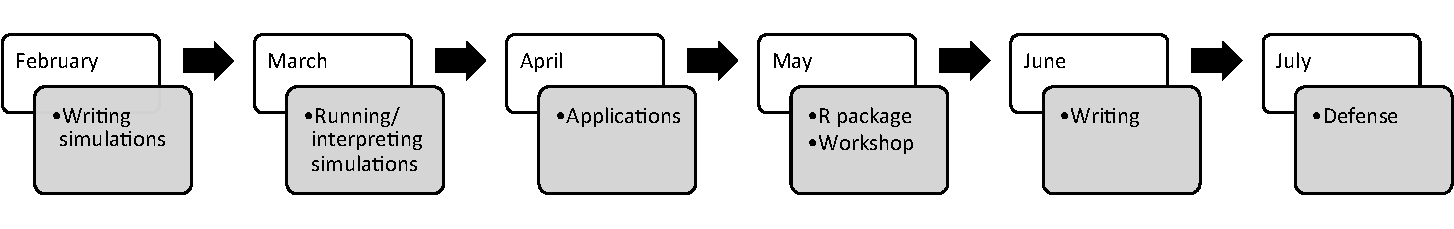
\includegraphics[width=4.5in]{Figures/Chapter05/timeline.pdf}
  \caption[My proposed dissertation timeline.]{\textit{My proposed dissertation timeline.}}
  \label{fig:timeline}
\end{figure}

%----------------------------------------------------------------------------------------

\section{Conclusion}

	To conclude, recursive partitioning methods provide an efficient way to perform exploratory data analysis in the social sciences. However, the behavior of these methods when multilevel data are present is not well understood. For my dissertation, I propose examining the performance of these methods under various simulation conditions commonly found in education research. With what I learn from the simulation results, I will apply these methods to three real data sets in order to perform exploratory data analysis in a data-driven way. Following this, I will create and share an R package and a set of best practices to help applied researchers implement these analytic tools in their own research. With this proposal, I hope to highlight the potential benefits of using recursive partitioning methods for efficient exploratory data analysis in the social sciences, especially with regard to multilevel applications in education research. 

